\documentclass[a4paper, 10pt]{article}

\usepackage[slovene]{babel}
\usepackage[utf8]{inputenc}
\usepackage[T1]{fontenc}

\usepackage{amsmath}  % razna okolja za poravnane enačbe ipd.
\usepackage{amsthm}   % definicije okolij za izreke, definicije, ...
\usepackage{amssymb}  % dodatni matematični simboli
\usepackage{xypic}    % paket za diagrame
\usepackage{lmodern}    % pisava
\usepackage{url}
\usepackage{xcolor}

\usepackage{hyperref}   % Paket za povezave znotraj dokumenta in hiper-povezave
\usepackage{makeidx}    % Za izdelavo stvarnega kazala

\usepackage{graphicx} % za vstavljanje slik
\usepackage{booktabs} % za lepše tabele
\usepackage{multirow} % za vnose v tabeli čez več vrstic
\usepackage{siunitx}  % za poravnavo na decimalni vejici v tabeli
\sisetup{output-decimal-marker={,},group-separator={.}}
\usepackage{listings} % za prikaz programske kode
\usepackage{pgfplots} % za risanje grafa funkcije
\usepackage{tikz}


% Definicija okoli za definicije
{\theoremstyle{definition}
\newtheorem{definicija}{Definicija}
}

% Definicija okolij izrek, posledica
{\theoremstyle{plain}
\newtheorem{izrek}{Izrek}
}


\begin{document}

\title{Primer LaTex dokumenta}
\author{Julija Brecl}
\date{9.\ 2.\ 2025}
% ali \date{} da se datum skrije
\maketitle

\begin{abstract}
    To je povzetek na začetku dokumenta.
\end{abstract}


\section{Prvo poglavje}
\subsection{podpoglavje}
\subsubsection{podpodpoglavje}
\paragraph{To je podpodpodrazdelek}

V tem odstavku so predstavljeni ukazi za poudarjanje in razčlenevanje besedila. To pomeni, da lahko določeno besedo zapišemo v \emph{kurzivi}, spet drugo pa morda \underline{podčrtamo}. Brez skrbi, obstajajo tudi črke, ki so \textbf{krepke}. Seveda se da besedo zapisati kot v izvorni \texttt{kodi}. Besedo lahko linearno damo v okolje \verb|vermatim|, kar izgleda takole. Pišemo lahko tudi v \textsf{sans-serifni pisavi} ali pa \textsc{kapitelkami},
denimo \textsc{Python}. Ležeča pisava \textsl{ni ista reč kot} \emph{poudarjena pisava}.

Takole napišemo `enojne' narekovaje. Poiščite ta dva znaka na tipkovnici. Dvoje narekovaje
pišemo ``takole''. Pravzaprav s tem dobimo angleške narekovaje. Slovenski narekovaji so
">takšni"< ali pa "`takšni"'.
Napačni načini pisanja narekovajev: znaka za levi in desni narekovaj nista enaka, zato se
\emph{ne} piše 'takole' ali ''takole''. Še posebej pa se ne piše "takole".

Ker ima vsak surjektivna funkcija $f : A \to B$ prerez,\footnote{takole se dela opombe} je svet lepši.



\section{Uporabna okolja}

% okolje za izvorno kodo?
\begin{verbatim}
    <profesor>
       <ime>Janez</ime>
    </profesor>
\end{verbatim}

% okolje za zapis izvorne kode
\begin{lstlisting}[language=Python,numbers=left,escapechar=|]
    def quickSort(arr):
        if len(arr) <= 1:
            return arr
        else:
            pivot = arr[0]
            for i in arr:
    a = quickSort(a)
\end{lstlisting}

% okolje za alineje
\begin{itemize}
    \item prva alineja
    \item druga  alineja seznama
    \item afina preslikava
\end{itemize}

% okolje za oštevilčene alineje
\begin{enumerate}
    \item prva oštevilčena alineja
    \item in zadnja 
\end{enumerate}

\begin{center}
    bla bla to je centralno centrirano besedilo\\
    tole je nova vrstica\\
    ki se zaključi z dvojno poševnico
\end{center}

% Levo poravnano besedilo
\begin{flushleft}
And no one showed us to the land\\
And no one knows the wheres or whys\\
But something stirs and something tries\\
And starts to climb towards the light
\end{flushleft}

% desno poravnano besedilo
\begin{flushright}
Strangers passing in the street\\
By chance two separate glances meet\\
And I am you and what I see is me\\
And do I take you by the hand\\
\end{flushright}

% tabela
\begin{center}
    \begin{tabular}{cl}
        znak & ukaz \\
        a & 1 \\
        b & 2 \\
        c & 3 \\
        d & 4 \\
    \end{tabular}
\end{center}

% tabele
\begin{table}[htp]
    \centering
    % kako se poravnajo podatki l-levo, r-desno in če so vmes rubričnice |
    \begin{tabular}{|l|r|r|}
    % zgornja okvirnica, v preglednicah uporabimo \toprule, \midrule in \bottomrule
    \hline 
    \textbf{Kandidat/Kandidatka}        & \textbf{Odstotek} & \textbf{Število glasov} \\ \hline
    Borut Pahor                & 47,07\%  & 348.938 \\ \hline
    Marjan Šarec               & 24,96\%  & 185.042 \\ \hline
    Romana Tomc                & 13,74\%  & 101.845 \\ \hline
    Ljudmila Novak             & 7,16\%   & 53.049 \\ \hline
    Andrej Šiško               & 2,22\%   & 16.463 \\ \hline
    Boris Popovič              & 1,79\%   & 13.277 \\ \hline
    dr.\ Maja Makovec Brenčič  & 1,72\%   & 12.734 \\ \hline
    Suzana Lara Krause         & 0,77\%   & 5.718 \\ \hline
    Angela (Angelca) Likovič   & 0,58\%   & 4.273 \\ \hline
    \end{tabular}
    \caption{Rezultati predsedniških volitev, kot bi jih prikazali z grdo razpredelnico, ki ima preveč črt.} 
    \label{tab:volitve-vanilla}
\end{table}

% citiranje
\begin{quote}
    Tole je okolje za daljši navedek iz nekega besedila nekega avtorja bla bla 
\end{quote}

\section{Vklučevanje slik}
% vklučevanje slik
\begin{figure}
    \centering
    
\includegraphics[width=0.5\textwidth]{muca.jpg}
    \caption{Prvi zadetek na Google za ``the cutest kitten in the world.''}
\end{figure}
% vklučevanje tikz grafik, potreben je paket tikz
\begin{center}
    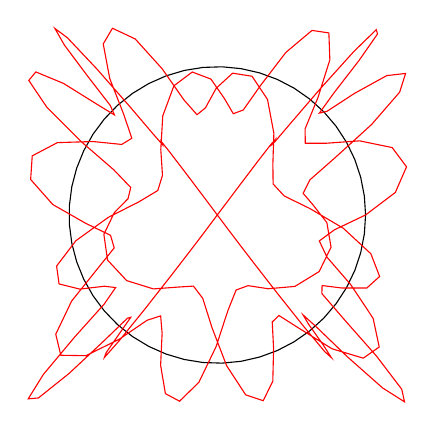
\begin{tikzpicture}
    \begin{axis}[
        trig format plots=rad,
        axis equal,
        hide axis
    ]
    \addplot [domain=0:2*pi, samples=50, black] ({cos(x)}, {sin(x)});
    \addplot [domain=0:2*pi,samples=200, red]({(1+0.3*sin(24*x))*cos(3*x)},{(1+0.3*sin(24*x))*sin(4*x)});
    \end{axis}
    \end{tikzpicture}
\end{center}


\section{Viri}
% Navajanje virov, ker smo uporabili paket \texttt{hyperref}, lahko na povezave kar kliknete:
\begin{description}
    \item[\href{http://www-lp.fmf.uni-lj.si/plestenjak/vaje/latex/lshort.pdf}{\emph{Ne najkrajši uvod v {\LaTeX}}}]
    Ravno pravšnji pregled {\LaTeX}a --- priporočamo!
  
    \item[\url{https://www.sharelatex.com/learn/Main_Page}]
    Naučite se LaTeX v 30 minutah!
\end{description}



\section{Matematika}
\label{sec:matematika}
% matematični način
\[ k_{1} \cdot u_{1} + k_{2} \]
za vsak realen pozitiven $x$ obstaja $k \in \mathbb{N}$, da je $0 < 1/k < x$.
$x_1, \ldots, x_n$
\[
  \frac{x_1 + \cdots + x_n}{n} \leq
  \sqrt{\frac{x_1^2 + \cdots + x_n^2}{n}},
\]

% poravnane in večvrstične enačbe
\subsection{enačbe} 
\begin{equation*}
    \mathcal{P} = \{ n \in \mathbb{N} \mid \text{$n$ je praštevilo} \}.
\end{equation*}

% neoštevilčena enačba *
\begin{equation*}
    x^2 + y^2 = 1
\end{equation*}
  %
  ali
  % oštevilčena enačba
\begin{equation}
    \label{eq:1}
    x^2 + y^2 = 1
\end{equation}

% več vrstic enačb
\begin{gather*}
    \log 2 = 1 - \frac{1}{2} + \frac{1}{3} - \frac{1}{4} + \cdots, \\
    \frac{2}{\frac{1}{x} + \frac{1}{y}} \leq \sqrt{x y} \leq \frac{x + y}{2}, \\
    \sum_{k = 1}^\infty \frac{1}{k^2} = \frac{\pi^2}{6}.
\end{gather*}

% Z okoljem \texttt{multtline} zapišemo daljšo izpeljavo čez več vrstic. Prva vrstica je
% poravnana levo, zadnja desno in vsem vmesne sredinsko:
\begin{multline*}
  1 + 2 + 3 + 4 + 5 + 6 + 7  = \\ 
  7 + 6 + 5 + 4 + 3 + 2 + 1 = \\
  1 + 2 + 3 + 4 + 5 + 6 + 7 = \\
  = 28
\end{multline*}

% poravnane vrstice, poravnajo se na &
\begin{align*}
    (x + y)^2 - (x - y)^2
    &= (x^2 + 2 x y + y^2) - (x^2 - 2 x y + y^2) \\
    &= x^2 + 2 x y + y^2 - x^2 + 2 x y - y^2 \\
    &= 2 x y + 2 x y \\
    &= 4 x y.
\end{align*}

% več poravnanih stolpcev, ločimo jih z znakom &
\begin{align*}
    3 + 5 &= 8
    &
    2 + 2 &= 4
    &
    1 + 1 &= 2
    \\
    3 + 7 &= 10
    &
    4 + 1 &= 5
    &
    2 + 3 &= 5
\end{align*}

% z okoljem cases obravnavamo primere
% funkcija podana po delih
\[
  f(x) =
  \begin{cases}
    -1 & \text{če $x < 1$,} \\
     x & \text{če $-1 \leq x \leq 1$,} \\
     1 & \text{če $1 < x$.}
  \end{cases}
\]

\subsection{Makroji}
% definicija novih ukazov (makroji)
\newcommand{\NN}{\mathbb{N}} % naravna števila
\[ \text{n} \in \NN\]

\subsection{oklepaji}
Poznamo več vrst oklepajev: $($ in $)$, $[$ in $]$, $\{$ in $\}$, $\langle$ in $\rangle$.


\subsection{Matrike}

\[
P =
\begin{bmatrix}
    1 & 2 & 3\\
    a & b & c
\end{bmatrix}
\]

\subsection{Izreki in dokazi}

\begin{definicija}
    \emph{Praštevilo} je tako naravno število $n$, večje od $1$, ki ni deljivo z nobenim
    naravnih šetvilom.
\end{definicija}

\begin{izrek}
    Vsaka zvezna funkcija na zaprtem intervalu doseže maksimum.
\end{izrek}


\section{Stvarno kazalo}
Stvarno kazalo%
\index{stvarno kazalo}%
je malo bolj komplicirana reč. V člankih ga običajno ne uporabljamo, za daljša besedila pa
pride prav. V tej datoteki vidite osnovno uporabo paketa \texttt{makeidx} za izdelavo
stvarnega kazala.

%% STVARNO KAZALO
\printindex


\subsection{Citati in reference}
\label{sec:citati}

Elementu, na katerega se sklicuješ moraš dodati ukaz label. Tam kjer se na to sklicuješ uporabiš ukaz ref in ime iz label oznake.
\ref{sec:citati}

Če se sklicujemo na stran uporabimo \pageref{sec:matematika} in če se sklicujemo na neko enačbo uporabimo ukaz \eqref{eq:1}.
Tam kjer hočemo citirati nek literaturni vir dodamo ukaz \cite{Tarski55} z naslovom dela ki je v dokumentu nekaj.bib

%% BIBLIOGRAFIJA
%% Najprej nastavimo stil bibliografije (plain, alpha, abbrv, ...)
\bibliographystyle{plain}
%% Datoteka za Bibtex
\bibliography{literatura}


\end{document}